\chapter{Model Accuracy Result for given 1 Year (2014)}
\label{ch:AccuracyResult}
In this chapter, all test result would be represented and discussed here. Most of those test results try to predict one year stock price. The addition result can be found in Appendix~\\


In this chapter, all result are about predict one year stock price, the average stock price data during this period is show in table~\ref{tb:avg20142015}. From 2014-01-06 to 2015-01-06, 248 transaction days in total.

\begin{table}[h]
	\centering
	\begin{tabular}{|l|l|l|l|}
		\hline
		\textbf{Stock Symbol} & \textbf{Average Price(HKD)} & \textbf{Stock Symbol} & \textbf{Average Price (HKD)} \\ \hline
		\textbf{0001.HK}      & 94.9379262096775       & \textbf{0006.HK}      & 68.62278225806452      \\ \hline
		\textbf{0002.HK}      & 63.25927419354843      & \textbf{0007.HK}      & 1.316129032258065      \\ \hline
		\textbf{0003.HK}      & 19.05447125000001      & \textbf{0008.HK}      & 4.466854838709676      \\ \hline
		\textbf{0004.HK}      & 55.95322580645161      & \textbf{0009.HK}      & 0.6356521739130431     \\ \hline
		\textbf{0005.HK}      & 80.08870967741933      & \textbf{0010.HK}      & 39.71733870967743      \\ \hline
	\end{tabular}
	\caption{Average Stock Price (from 2014-01-06 to 2015-01-06)}
	\label{tb:avg20142015}
\end{table}

\section{Using 4 years historical data}
\label{sec:4predict}

Training data is sampled from 2010-01-06 to 2014-01-05, 986 transaction days in total.\\


Comparison of different measurements is in figure~\ref{fg:4yearpredict1} and \ref{fg:4yearpredict2}. Average CDC and MAPE information can be found in table~\ref{tb:averageCDC1} and \ref{tb:averageMAPE1} respectively.\\

\begin{table}[h]
	\centering
	\begin{tabular}{|l|l|}
		\hline
		\textbf{Algorithm} & \textbf{Average CDC} \\ \hline
		\textbf{ANN} & 47.63\% \\ \hline
		\textbf{Linear Regression} & 47.31\% \\ \hline
		\textbf{Random Forest} & 64.27\% \\ \hline
		\textbf{\begin{tabular}[c]{@{}l@{}}Linear Regression \\ + Logistic Regression\end{tabular}} & 60.17\% \\ \hline
		\textbf{Random Forest + SVM} & 60.25\% \\ \hline
		\textbf{ANN + Random Forest} & 65.31\% \\ \hline
	\end{tabular}
	\caption{Average CDC of using 4 years historical data}
	\label{tb:averageCDC1}
\end{table}

\begin{table}[h]
	\centering
	\begin{tabular}{|l|l|}
		\hline
		\textbf{Algorithm} & \textbf{Average MAPE} \\ \hline
		\textbf{ANN} & 1.45\% \\ \hline
		\textbf{Linear Regression} & 1.46\% \\ \hline
		\textbf{Random Forest} & 1.56\% \\ \hline
		\textbf{\begin{tabular}[c]{@{}l@{}}Linear Regression \\ + Logistic Regression\end{tabular}} & 9.85\% \\ \hline
		\textbf{Random Forest + SVM} & 2.98\% \\ \hline
		\textbf{ANN + Random Forest} & 2.76\% \\ \hline
	\end{tabular}
	\caption{Average MAPE of using 4 years historical data}
	\label{tb:averageMAPE1}
\end{table}

The best learning algorithm under this circumstance is Random Forest, which has the second best CDC (In figure~\ref{fg:4yearpredict2}.b and table~\ref{tb:averageCDC1} the best algorithm is a combined method whose trend model is also based on Random Forest) and lowest error in amount prediction. And as both linear classifiers, the CDC result of Logistic Regression and SVM are almost same\\


For combination method, random forest algorithm is also the best model to predict stock price change amount. The performance of classifiers is also acceptable.


\section{Using 3 years historical data}
\label{sec:3predict}
Training data is sampled from 2011-01-06 to 2014-01-05, 736 transaction days in total.\\


Comparison of different measurements is in figure~\ref{fg:3yearpredict1} and \ref{fg:3yearpredict2}. Average CDC and MAPE information can be found in table~\ref{tb:averageCDC2} and \ref{tb:averageMAPE2} respectively.\\

\begin{table}[h]
	\centering
	\begin{tabular}{|l|l|}
		\hline
		\textbf{Algorithm} & \textbf{Average CDC} \\ \hline
		\textbf{ANN} & 46.55\% \\ \hline
		\textbf{Linear Regression} & 46.92\% \\ \hline
		\textbf{Random Forest} & 63.83\% \\ \hline
		\textbf{\begin{tabular}[c]{@{}l@{}}Linear Regression \\ + Logistic Regression\end{tabular}} & 55.93\% \\ \hline
		\textbf{Random Forest + SVM} & 55.90\% \\ \hline
		\textbf{ANN + Random Forest} & 65.99\% \\ \hline
	\end{tabular}
	\caption{Average CDC of using 3 years historical data}
	\label{tb:averageCDC2}
\end{table}

\begin{table}[h]
	\centering
	\begin{tabular}{|l|l|}
		\hline
		\textbf{Algorithm} & \textbf{Average MAPE} \\ \hline
		\textbf{ANN} & 1.35\% \\ \hline
		\textbf{Linear Regression} & 1.29\% \\ \hline
		\textbf{Random Forest} & 1.66\% \\ \hline
		\textbf{\begin{tabular}[c]{@{}l@{}}Linear Regression \\ + Logistic Regression\end{tabular}} & 7.79\% \\ \hline
		\textbf{Random Forest + SVM} & 1.65\% \\ \hline
		\textbf{ANN + Random Forest} & 3.34\% \\ \hline
	\end{tabular}
	\caption{Average MAPE of using 3 years historical data}
	\label{tb:averageMAPE2}
\end{table}

Composed learning model performed better in CDC test (in table~\ref{tb:averageCDC2}). Two linear classifiers share similar performance in this test. ANN and Linear Regression are also not trustworthy method to predict stock change direction\\

Random Forest alone and Linear + Logsitic Regression model turns out to be an unreliable choice to predict stock price in this test for some stock (like 0009.HK and 0007.HK). However, almost every method reach its worst performance when handle this two stocks, which on the other way shows that those model are not suitable for stock with average price less than.

\section{Using 2 years historical data}
\label{sec:2predict}
Training data is sampled from 2012-01-06 to 2014-01-05, 490 transaction days in total.\\

Comparison of different measurements is in figure~\ref{fg:2yearpredict1} and \ref{fg:2yearpredict2}. Average CDC and MAPE information can be found in table~\ref{tb:averageCDC3} and \ref{tb:averageMAPE3} respectively.

\begin{table}[h]
	\centering
	\begin{tabular}{|l|l|}
		\hline
		\textbf{Algorithm} & \textbf{Average CDC} \\ \hline
		\textbf{ANN} & 46.29\% \\ \hline
		\textbf{Linear Regression} & 47.22\% \\ \hline
		\textbf{Random Forest} & 56.79\% \\ \hline
		\textbf{\begin{tabular}[c]{@{}l@{}}Linear Regression \\ + Logistic Regression\end{tabular}} & 62.54\% \\ \hline
		\textbf{Random Forest + SVM} & 62.50\% \\ \hline
		\textbf{ANN + Random Forest} & 59.19\% \\ \hline
	\end{tabular}
	\caption{Average CDC of using 2 years historical data}
	\label{tb:averageCDC3}
\end{table}

\begin{table}[h]
	\centering
	\begin{tabular}{|l|l|}
		\hline
		\textbf{Algorithm} & \textbf{Average MAPE} \\ \hline
		\textbf{ANN} & 1.33\% \\ \hline
		\textbf{Linear Regression} & 1.29\% \\ \hline
		\textbf{Random Forest} & 3.04\% \\ \hline
		\textbf{\begin{tabular}[c]{@{}l@{}}Linear Regression \\ + Logistic Regression\end{tabular}} & 7.54\% \\ \hline
		\textbf{Random Forest + SVM} & 2.15\% \\ \hline
		\textbf{ANN + Random Forest} & 3.74\% \\ \hline
	\end{tabular}
	\caption{Average MAPE of using 2 years historical data}
	\label{tb:averageMAPE3}
\end{table}

When it comes to two years data forecast, Random Forest works not so well in predict data. The best method in this test is to use Logistic Regression or SVM (both CDC above 60\%) to predict stock change direction and use ANN or Linear Regression to Predict stock price change amount.\\

The worst stock performance in there 0009.HK and 0007.HK, none of the prediction method can achieve 50\% CDC in predicting these two stocks. 


\section{Using 1 year historical data}
\label{sec:1predict}
Training data is sampled from 2013-01-06 to 2014-01-05, 490 transaction days in total.\\

Comparison of different measurements is in figure~\ref{fg:1yearpredict1} and \ref{fg:1yearpredict2}. Average CDC and MAPE information can be found in table~\ref{tb:averageCDC4} and \ref{tb:averageMAPE4} respectively.

\begin{table}[h]
	\centering
	\begin{tabular}{|l|l|}
		\hline
		\textbf{Algorithm} & \textbf{Average CDC} \\ \hline
		\textbf{ANN} & 45.66\% \\ \hline
		\textbf{Linear Regression} & 47.22\% \\ \hline
		\textbf{Random Forest} & 52.98\% \\ \hline
		\textbf{\begin{tabular}[c]{@{}l@{}}Linear Regression \\ + Logistic Regression\end{tabular}} & 60.50\% \\ \hline
		\textbf{Random Forest + SVM} & 60.68\% \\ \hline
		\textbf{ANN + Random Forest} & 52.20\% \\ \hline
	\end{tabular}
	\caption{Average CDC of using 2 year historical data}
	\label{tb:averageCDC4}
\end{table}

\begin{table}[h]
	\centering
	\begin{tabular}{|l|l|}
		\hline
		\textbf{Algorithm} & \textbf{Average MAPE} \\ \hline
		\textbf{ANN} & 2.01\% \\ \hline
		\textbf{Linear Regression} & 1.39\% \\ \hline
		\textbf{Random Forest} & 2.20\% \\ \hline
		\textbf{\begin{tabular}[c]{@{}l@{}}Linear Regression \\ + Logistic Regression\end{tabular}} & 6.50\% \\ \hline
		\textbf{Random Forest + SVM} & 2.49\% \\ \hline
		\textbf{ANN + Random Forest} & 5.27\% \\ \hline
	\end{tabular}
	\caption{Average MAPE of using 1 year historical data}
	\label{tb:averageMAPE4}
\end{table}

Linear Regression is the best method in here to predict stock change amount, and SVM is the best method to predict stock change direction. 

\begin{figure}[h]
	\centering
	\subfigure[RMSE]{
		\centering
		\includegraphics[width=.8\textwidth]{Result/20102015/RMSE}
	}
	\subfigure[MSE]{
		\centering
		\includegraphics[width=.8\linewidth]{Result/20102015/MSE}
	}
	\caption{Testing result of using 4 years historical data}
	\label{fg:4yearpredict1}
\end{figure}

\begin{figure}[h]
	\centering
	\subfigure[ME]{
		\centering
		\includegraphics[width=.8\textwidth]{Result/20102015/ME}
	}
	\subfigure[HMSE]{
		\centering
		\includegraphics[width=.8\linewidth]{Result/20102015/HMSE}
	}
	\caption{Testing result of using 4 years historical data (continue)}
	\label{fg:4yearpredict2}
\end{figure}

\begin{figure}[h]
	\centering
	\subfigure[RMSE]{
		\centering
		\includegraphics[width=.8\textwidth]{Result/20112015/RMSE}
	}
	\subfigure[ME]{
		\centering
		\includegraphics[width=.8\linewidth]{Result/20112015/ME}
	}
	\caption{Testing result of using 3 year as test result}
	\label{fg:3yearpredict1}
\end{figure}

\begin{figure}[h]
	\centering
	\subfigure[MSE]{
		\centering
		\includegraphics[width=.8\textwidth]{Result/20112015/MSE}
	}
	\subfigure[HMSE]{
		\centering
		\includegraphics[width=.8\linewidth]{Result/20112015/HMSE}
	}
	\caption{Testing result of using 3 year as test result (continue)}
	\label{fg:3yearpredict2}
\end{figure}

\begin{figure}[h]
	\centering
	\subfigure[ME]{
		\centering
		\includegraphics[width=.8\linewidth]{Result/20122015/ME}
	}
	\subfigure[MAPE]{
		\centering
		\includegraphics[width=.8\textwidth]{Result/20122015/MAPE}
	}
	\caption{Testing result of using 2 years historical data}
	\label{fg:2yearpredict1}
\end{figure}


\begin{figure}[h]
	\centering
	\subfigure[RMSE]{
		\centering
		\includegraphics[width=.8\textwidth]{Result/20122015/RMSE}
	}
	\subfigure[CDC]{
		\centering
		\includegraphics[width=.8\linewidth]{Result/20122015/CDC}
	}
	\caption{Testing result of using 2 years historical data (continue)}
	\label{fg:2yearpredict2}
\end{figure}

\begin{figure}[h]
	\centering
	\subfigure[ME]{
		\centering
		\includegraphics[width=.8\linewidth]{Result/20132015/ME}
	}
	\subfigure[MAPE]{
		\centering
		\includegraphics[width=.8\textwidth]{Result/20132015/MAPE}
	}
	\caption{Testing result of using 1 year historical data}
	\label{fg:1yearpredict1}
\end{figure}


\begin{figure}[h]
	\centering
	\subfigure[RMSE]{
		\centering
		\includegraphics[width=.8\textwidth]{Result/20132015/RMSE}
	}
	\subfigure[CDC]{
		\centering
		\includegraphics[width=.8\linewidth]{Result/20132015/CDC}
	}
	\caption{Testing result of using 1 year historical data (continue)}
	\label{fg:1yearpredict2}
\end{figure}

\section{Summary}
The above test concludes that,
\begin{enumerate}
	\item Classification methods perform better than just Regression alone.
	\item Predict the change amount of stock price works worse than use one method to predict the stock price directly.
	\item All methods does not performs well in predict stock with very small price (Like 0007.HK and 0009.HK).
	\item Two years seems to be the most reliable choice for model training period.
	\item The difference between may also means that the data this study chosen is more suitable to predict this type of stock (like 0002.HK, many method reach its best performance while predict it), does these method still works well in predict its price during other period? Or this price prediction method would also works well for company of same style as 0002.HK? 
\end{enumerate}

It is clear that the above test is not strong enough to support the above conclusions, more test is still needed

